\chapter{이징 자석에서 액체--기체 임계성으로}

\lectureoverview{액체--기체 전이는 예상 밖의 경로로 살펴볼 수 있다. 먼저 이징 자석의 평균장 설명을 마무리하고 공존선과 임계점을 찾은 다음, 위쪽 스핀을 점유된 격자 사이트로 다시 해석한다. 이렇게 얻은 격자 기체에는 하드코어 배제와 단거리 인력이 있고, 자기장에 따라 화학 퍼텐셜이 조절되며, 상도는 정확히 동일하다. 정규 강의는 임계 거동과 보편성으로 끝난다. 별도의 강의 후 토론에서는 물리학자들이 미세 조정이라 부르는 것이 무엇인지, 선택 효과가 설명에 어떻게 들어갈 수 있는지, 그리고 그런 추론이 메커니즘 및 가능한 검증 방법과 함께할 때에만 왜 유용한지를 살펴본다.}

\section{끓는 물을 자석에서부터 살펴보는 이유}

끓는 물은 우리가 이해하고자 하는 익숙한 현상이다. 액체가 기체로 바뀌면서 밀도가 급격히 변한다. 보통은 반데르발스 방정식으로 이 현상을 설명한다. 여기서는 다른 경로를 택한다. 이징 자석으로 돌아가 평균장 설명을 마무리하고, 같은 모형을 유체로 해석할 수 있음을 알아본다.

이것은 단순히 그럴듯한 비유에 그치지 않는다. 변수를 올바르게 바꾸면 이징 자석과 격자 기체는 동일한 통계역학계가 된다. 자화는 입자 밀도로, 외부 자기장은 화학 퍼텐셜로, 자기 공존선은 액체--기체 공존선으로 바뀐다. 이러한 대응을 통해 서로 달라 보이는 두 물질이 왜 같은 임계 거동을 보일 수 있는지 알 수 있다.

평균장 이론은 저차원에서 정확한 수치 답을 주지 못한다. 1차원에서는 정확해가 금지하는 상전이까지 예측한다. 여기서 평균장 이론의 가치는 구조를 드러내는 데 있다. 2차원과 3차원에서는 올바른 질서변수와 경쟁하는 상, 임계 종점, 무한소 편향이 한 상을 선택하는 방식을 보여준다. 모든 사이트에 최근접 이웃이 6개인 3차원에서 이웃들의 값을 평균으로 대체하는 것만으로도 유용한 정성적 그림을 얻을 수 있다.

\section{이징 에너지의 계산}

초입방 격자의 모든 사이트에 두 상태를 갖는 스핀을 하나씩 둔다.
\begin{equation}
\sigma_i=\pm1.
\end{equation}
해밀토니안은 다음과 같다.
\begin{equation}
\mathcal H
=-J\sum_{\langle ij\rangle}\sigma_i\sigma_j
+h\sum_i\sigma_i,
\qquad J>0.
\label{eq:ising-hamiltonian}
\end{equation}
표기법이 중요하다. 첫 번째 합은 최근접 이웃 \emph{결합}에 대한 합이고, 두 번째 합은 \emph{사이트}에 대한 합이다. 하나의 결합은 양 끝점에서 각각 세지 않고 한 번만 센다.

단일 결합의 경우,
\begin{equation}
E_{ij}=-J\sigma_i\sigma_j.
\end{equation}
평행한 스핀의 에너지는 \(-J\)이고, 반평행한 스핀의 에너지는 \(+J\)이다. 따라서 결합을 끊는 데 드는 에너지는
\begin{equation}
\Delta E_{\rm bond}=+J-(-J)=2J.
\label{eq:broken-bond}
\end{equation}
각 결합의 절대 에너지보다 \(2J\)라는 차이가 볼츠만 가중치의 상대적 크기를 좌우한다. 모든 배치에 상수를 더해도 확률은 변하지 않는다.

\begin{classroomqa}
\audiencequestion{해밀토니안에 왜 서로 다른 합이 두 개 있나요?}
\lecturerresponse{교환 에너지는 이웃한 두 사이트 한 쌍에 속하므로 결합 \(\langle ij\rangle\)에 대해 합한다. 자기장은 각 스핀에 독립적으로 작용하므로 사이트 \(i\)에 대해 합한다. 이 두 셈을 혼동하면 평균장에서 중요한 2의 인자가 바로 잘못 들어간다. \lecturetimestamp{00:08:04--00:08:45}}
\end{classroomqa}

\begin{classroomqa}
\audiencequestion{\(J\)를 키우면 단순히 모든 에너지가 더 음수가 되나요?}
\lecturerresponse{정렬된 배치와 정렬되지 않은 배치 사이의 에너지 차이가 커진다. 에너지의 영점은 임의로 정할 수 있다. 물리적으로 중요한 것은 결합을 끊는 데 \(2J\)가 든다는 점이다. 따라서 양의 \(J\)가 클수록 온도가 고정되어 있을 때 열적 무질서가 덜 유리해진다. \lecturetimestamp{00:08:47--00:10:17}}
\end{classroomqa}

\(d\)차원의 무한 또는 주기적 초입방 격자에서는 모든 사이트에 이웃이 \(2d\)개 있다. 모든 \(N\)사이트에서 세면 각 결합을 두 번 세게 되므로,
\begin{equation}
N_{\rm links}=\frac{(2d)N}{2}=dN.
\label{eq:number-links}
\end{equation}
따라서 정렬된 배치의 교환 에너지는 \(-JdN\)이다. 경계 사이트는 표면 항만큼 이 값을 바꾸지만, 열역학적 극한에서는 \(N\)에 비해 무시할 수 있다. \(h=0\)일 때 완전히 정렬된 두 상태는 축퇴되어 있다.

자기장 항은 이후에도 일관되게 따를 부호 규약을 정한다. 식~\eqref{eq:ising-hamiltonian}에서 양의 \(h\)는 사이트 에너지를 \(\sigma=-1\)일 때 더 낮게 만든다. 따라서 \(h>0\)는 음의 자화를, \(h<0\)는 양의 자화를 선호한다. \(-h\sum_i\sigma_i\)로 쓰면 이 규약을 뒤집을 수 있다. 물리적 내용은 바뀌지 않지만, 이후의 부호를 모두 함께 바꿔야 한다.

\begin{classroomqa}
\audiencequestion{해밀토니안에 \(J\)와 \(h\)만 있는데 온도는 어디에 들어가나요?}
\lecturerresponse{온도는 볼츠만 인자 \(e^{-\beta\mathcal H}\)를 통해 들어가며, 여기서는 \(\beta=1/T\)이고 단위는 \(k_{\rm B}=1\)이다. 따라서 무차원량은 \(\beta J\)와 \(\beta h\)이다. \lecturetimestamp{00:13:07--00:13:43}}
\end{classroomqa}

\section{이웃의 평균장 속 단일 스핀}

경계에서 멀리 떨어진 스핀 하나를 고르자. 이 스핀에는 최근접 이웃이 \(2d\)개 있다. 평균장 이론에서는 요동하는 각 이웃을 동일한 평균값으로 대체한다.
\begin{equation}
m=\expect{\sigma}.
\end{equation}
선택한 스핀 \(\sigma\)과 관련된 교환 에너지는 이제 다음과 같다.
\begin{equation}
-J\sigma\sum_{\text{\(2d\) neighbors}}\sigma_j
\;\longrightarrow\;-2dJm\,\sigma.
\end{equation}
외부 자기장 항을 더하면 유효한 단일 스핀 에너지는
\begin{equation}
\mathcal H_{\rm mf}(\sigma)=(-2dJm+h)\sigma.
\label{eq:mean-field-one-spin}
\end{equation}
이때 \(2d\)라는 인자가 중요하다. 중심 스핀 그림을 그릴 때 빠뜨리기 쉽지만, 판서 유도 과정에서 명시적으로 다시 넣었다.

\begin{figure}[ht]
\centering
\includegraphics[width=0.84\textwidth]{lecture_10_figure_02.png}
\caption{평균장 이웃들로 둘러싸인 중심 스핀, 한 스핀의 에너지, 그리고 전개 중인 자기일관성 방정식.}
\lectureframe{00:17:57}
\end{figure}

단일 스핀의 분배함수는
\begin{align}
z_{\rm mf}
&=\sum_{\sigma=\pm1}
\exp\!\left[-\beta(-2dJm+h)\sigma\right] \\
&=2\cosh\!\left[\beta(2dJm-h)\right].
\end{align}
평균 스핀은
\begin{align}
\expect{\sigma}
&=\frac{\sum_{\sigma=\pm1}\sigma
 e^{\beta(2dJm-h)\sigma}}
{\sum_{\sigma=\pm1}e^{\beta(2dJm-h)\sigma}} \\
&=\tanh\!\left[\beta(2dJm-h)\right].
\end{align}
이다. 그런데 선택한 스핀은 평균을 \(m\)라고 둔 이웃들을 대표하는 스핀이어야 한다. 따라서 자기일관 조건은
\begin{equation}
\boxed{m=\tanh\!\left[\beta(2dJm-h)\right].}
\label{eq:mean-field-self-consistency}
\end{equation}
이 비선형 방정식 하나로 다중 스핀 문제를 평균장 문제로 축약할 수 있다.

\begin{classroomqa}
\audiencequestion{왼쪽의 평균은 왜 모든 이웃에 대입한 것과 같은 \(m\)인가요?}
\lecturerresponse{그 등식이 바로 근사다. 균질한 벌크 상태를 가정하고 실제 환경을 그 평균으로 대체한 다음, 그 환경에 놓인 중심 스핀을 계산하고, 계산된 평균이 가정한 환경을 재현하도록 요구한다. 해는 자기일관적인 벌크 상태다. \lecturetimestamp{00:16:28--00:18:00}}
\end{classroomqa}

다음을 도입하자.
\begin{equation}
y=2\beta dJm.
\label{eq:y-definition}
\end{equation}
\(\beta=1/T\)이므로,
\begin{equation}
m=\frac{yT}{2dJ},
\end{equation}
식~\eqref{eq:mean-field-self-consistency}은 다음과 같이 된다.
\begin{equation}
\boxed{\frac{yT}{2dJ}=\tanh(y-\beta h).}
\label{eq:reduced-mean-field}
\end{equation}

\begin{figure}[ht]
\centering
\includegraphics[width=0.82\textwidth]{lecture_10_figure_03.png}
\caption{\(y=2\beta dJm\)를 도입한 뒤 얻는 축약 자기일관성 방정식. 그래프로 풀 준비가 되어 있다.}
\lectureframe{00:24:42}
\end{figure}

\begin{classroomqa}
\audiencequestion{자기장은 왜 \(y-\beta h\)로 나타나며, 양의 자기장은 어떤 스핀을 선호하나요?}
\lecturerresponse{우리 해밀토니안에는 \(+h\sigma\)가 들어 있다. 따라서 볼츠만 지수는 \(\beta(2dJm-h)\sigma\)이며, 쌍곡탄젠트에는 \(y-\beta h\)가 들어간다. 양의 \(h\)는 \(\sigma=-1\)를 선호한다. 해밀토니안을 \(-h\sigma\)로 정의하면 \(h\)가 들어가는 모든 항의 부호가 바뀌고 상도는 수평 방향으로 반사된다. \lecturetimestamp{00:18:17--00:20:00}}
\end{classroomqa}

\section{그래프 해와 퀴리점}

\(h=0\)로 두자. 다음 두 함수의 교점을 찾아야 한다.
\begin{equation}
\frac{T}{2dJ}y
\qquad\text{and}\qquad
\tanh y.
\end{equation}
첫 번째는 원점을 지나는 직선이고, 두 번째는 홀함수이며 포화되는 곡선이다. 고온에서는 직선의 기울기가 크므로 교점은 \(y=0\) 하나뿐이고, 따라서 \(m=0\)이다. 온도가 내려가면 직선의 기울기는 작아진다. 직선과 쌍곡탄젠트 곡선이 원점에서 접할 때 임계 온도에 도달한다.

\begin{figure}[ht]
\centering
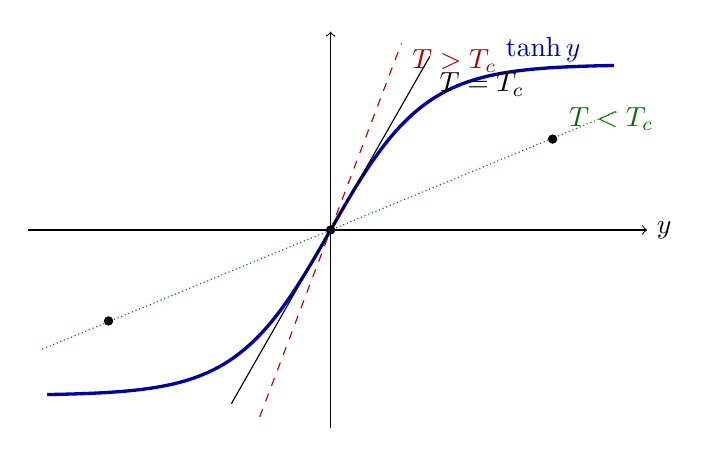
\begin{tikzpicture}[x=1.2cm,y=2.1cm]
\draw[->] (-3.2,0) -- (3.35,0) node[right] {$y$};
\draw[->] (0,-1.2) -- (0,1.2);
\draw[very thick,blue!65!black,domain=-3:3,samples=120]
  plot (\x,{tanh(\x)});
\node[blue!65!black,above] at (2.25,0.96) {$\tanh y$};
\draw[dashed,red!70!black] (-0.75,-1.13) -- (0.75,1.13);
\node[red!70!black,right] at (0.76,1.02) {$T>T_c$};
\draw[black] (-1.05,-1.05) -- (1.05,1.05);
\node[right] at (1.05,0.88) {$T=T_c$};
\draw[densely dotted,green!45!black] (-3.05,-0.72) -- (3.05,0.72);
\node[green!45!black,right] at (2.42,0.67) {$T<T_c$};
\fill (-2.35,-0.55) circle (1.7pt);
\fill (0,0) circle (1.7pt);
\fill (2.35,0.55) circle (1.7pt);
\end{tikzpicture}
\caption{영자기장에서의 평균장 방정식. \(T_c\)보다 낮은 온도에서 두 비영 교점은 안정한 자화 상을 나타낸다. 영 해도 대수적으로는 여전히 존재하지만 불안정하다.}
\label{fig:mean-field-intersections}
\end{figure}

다음이 성립하므로,
\begin{equation}
\left.\frac{d}{dy}\tanh y\right|_{y=0}=1,
\end{equation}
접선 조건은
\begin{equation}
\frac{T_c}{2dJ}=1.
\end{equation}
이다. 따라서 평균장 이론은 다음을 예측한다.
\begin{equation}
\boxed{T_c^{\rm MF}=2dJ.}
\label{eq:sm10-mean-field-tc}
\end{equation}
이 온도 아래에는 0이 아닌 안정한 해가 두 개, \(\pm m_0(T)\) 존재한다. \(m=0\)라는 해도 여전히 방정식을 만족하지만, 더 이상 안정한 평형은 아니다. 계는 대칭 관계에 있는 두 자화 상태 중 하나를 택한다.

\begin{classroomqa}
\audiencequestion{}가 퀴리 온도인가요?\lecturerresponse{
그렇다. 강자성체에서 자발 자화가 사라지는 온도는 관례적으로 퀴리 온도라고 부른다. 여기서 \(2dJ\)는 평균장 값이며, 저차원계의 정확한 결과는 아니다. \lecturetimestamp{00:28:19--00:28:57}}
\end{classroomqa}

전이점 근처에서 쌍곡탄젠트를 전개하면 다음과 같다:
\begin{equation}
\tanh y=y-\frac{y^3}{3}+O(y^5).
\end{equation}
\(h=0\)에서 방정식~\eqref{eq:reduced-mean-field}은 다음을 준다.
\begin{equation}
\left(1-\frac{T}{T_c}\right)y-\frac{y^3}{3}+O(y^5)=0.
\end{equation}
따라서 영이 아닌 가지는 다음과 같이 거동한다.
\begin{equation}
y^2\simeq3\left(1-\frac{T}{T_c}\right),
\qquad
m\propto(T_c-T)^{1/2}.
\label{eq:mf-beta-exponent}
\end{equation}
제곱근은 평균장 임계 지수다. 그 정확한 값은 저차원에서는 유지되지 않지만, 끝점에서 질서 매개변수가 연속적으로 사라지는 현상은 유지된다.

\section{온도--자기장 평면과 가지의 선택}

물질은 \(J\)를 정하고, 실험자는 \(T\)와 \(h\)를 바꿀 수 있다. 따라서 \(T\)--\(h\) 평면에 상도를 그리는 것이 자연스럽다. \(T_c\) 아래에서는 아무리 작은 자기장이라도 자화 가지 둘 중 하나를 선택한다. 여기서 정한 부호 규약에 따르면 \(h<0\)는 \(m>0\)를 선택하고, \(h>0\)는 \(m<0\)를 선택한다.

절대영도에서는 스핀이 완전히 정렬되어 있으므로 \(m=\pm1\)이다. 고온에서는 자기장이 0일 때 평균이 \(m=0\)이다. \(h=0\)을 따라 임계점에 접근하면 크기 \(m_0(T)\)가 연속적으로 0으로 감소한다. 그러나 \(T<T_c\)를 고정하고 \(h=0\)을 가로지르면 \(+m_0(T)\)에서 \(-m_0(T)\)로 불연속적으로 바뀐다.

\begin{figure}[ht]
\centering
\includegraphics[width=0.90\textwidth]{lecture_10_figure_06.png}
\caption{\(T\)--\(h\) 평면의 공존선과 \(T_c\)보다 낮은 고정 온도에서의 자화 가지.}
\lectureframe{00:39:30}
\end{figure}

\begin{figure}[ht]
\centering
\resizebox{\linewidth}{!}{%
\begin{tikzpicture}[x=1.25cm,y=1.15cm]
\begin{scope}
\draw[->] (-2.45,0) -- (2.55,0) node[right] {$h$};
\draw[->] (0,0) -- (0,3.7) node[above] {$T$};
\draw[very thick,red!70!black] (0,0) -- (0,2.35);
\fill[red!70!black] (0,2.35) circle (2.3pt);
\node[right] at (0.08,2.35) {$T_c$};
\node at (-1.25,1.05) {$m>0$};
\node at (1.25,1.05) {$m<0$};
\draw[->,rounded corners,blue!65!black] (-1.65,0.85) -- (-1.65,3.02)
 -- (1.65,3.02) -- (1.65,0.85);
\node[blue!65!black] at (0,3.35) {continuous path};
\end{scope}
\begin{scope}[xshift=7.0cm,yshift=1.55cm]
\draw[->] (-2.5,0) -- (2.5,0) node[right] {$h$};
\draw[->] (0,-1.35) -- (0,1.4) node[above] {$m$};
\draw[very thick,blue!65!black]
  (-2.2,1.05) .. controls (-0.75,1.03) and (-0.2,0.75) .. (-0.08,0.62);
\draw[very thick,blue!65!black]
  (0.08,-0.62) .. controls (0.2,-0.75) and (0.75,-1.03) .. (2.2,-1.05);
\draw[dashed] (0,0.62) -- (0,-0.62);
\fill (0,0.62) circle (1.8pt);
\fill (0,-0.62) circle (1.8pt);
\node at (0,-1.75) {\(T<T_c\)};
\end{scope}
\end{tikzpicture}
}
\caption{\(T<T_c\)를 고정하면 자화는 공존선을 가로질러 불연속적으로 도약한다. 두 매개변수 전체 평면에서는 임계점을 돌아가는 경로를 따라 두 상을 연속적으로 연결할 수 있다.}
\label{fig:ising-phase-plane}
\end{figure}

\begin{classroomqa}
\audiencequestion{\(T_c\) 아래에서 자기장이 정확히 0이면 어떻게 되나요?}
\lecturerresponse{이상적인 무한계에는 동등하게 안정한 순수상이 두 개 있다. 아무리 작은 잔류 편향이나 경계 조건, 또는 준비 과정에 따른 요동이라도 두 상 중 하나를 선택한다. 열역학적 불연속성은 이 부호 규약에서 한쪽 극한 \(m(T,0^-)=+m_0(T)\)과 다른 쪽 극한 \(m(T,0^+)=-m_0(T)\)으로 표현된다. \lecturetimestamp{00:35:04--00:37:10}}
\end{classroomqa}

\begin{classroomqa}
\audiencequestion{이 현상이 히스테리시스와 같은 것인가요?}
\lecturerresponse{히스테리시스는 준안정성과 실제 계가 가지를 바꿀 때 나타나는 이력 의존적 지연을 뜻한다. 서로 관련은 있지만, 평형 상도만으로는 다룰 수 없는 동역학이 필요하므로 여기서는 전개하지 않는다. \lecturetimestamp{00:37:11--00:37:20}}
\end{classroomqa}

\begin{classroomqa}
\audiencequestion{불연속을 가로지르지 않고 양의 상과 음의 상을 이을 수 있나요?}
\lecturerresponse{가능하다. 온도를 \(T_c\)보다 높인 뒤 그 온도에서 자기장의 부호를 바꾸고, 다시 온도를 낮추면 된다. 이 경로는 종점을 돌아가므로 자화가 연속적으로 변한다. 불연속적인 도약을 피할 수 없는 경우는 \(T<T_c\)에서 \(h=0\)를 고정한 채 그 선을 가로지를 때뿐이다. \lecturetimestamp{00:37:20--00:38:15}}
\end{classroomqa}

\begin{classroomqa}
\audiencequestion{자화는 \(h\)이 영에 가까워질 때마다 영에 가까워지는가?}
\lecturerresponse{임계 온도 \(T_c\)보다 낮은 일반적인 온도에서는 그렇지 않다. 그 온도에서는 양쪽 극한값이 영이 아니다. 자발 자화는 임계 온도 자체에 접근할 때에만 영에 가까워진다. \lecturetimestamp{00:38:29--00:39:45}}
\end{classroomqa}

\section{투과성 상자와 화학 퍼텐셜}

이제 자석을 떠나 입자에서부터 다시 시작하자. 주변 공간보다 퍼텐셜 에너지가 낮은 영역을 생각해 보자. 벽은 투과성이어서 입자가 드나들 수 있다. 내부 에너지가 바깥보다 \(\mu\)만큼 낮다면, 상자 안의 점유에는 상대 볼츠만 인자 \(e^{\beta\mu}\)가 곱해진다. 우물의 깊이를 더하거나 얕게 하면 상자 안 입자의 평균 개수가 달라진다.

\begin{figure}[ht]
\centering
\includegraphics[width=0.84\textwidth]{lecture_10_figure_07.png}
\caption{투과성 상자를 퍼텐셜 우물로 나타낸 그림. 안팎의 에너지 차이가 입자들이 상자 안에 존재하려는 선호도를 결정한다.}
\lectureframe{00:41:30}
\end{figure}

\begin{figure}[ht]
\centering
\resizebox{\linewidth}{!}{%
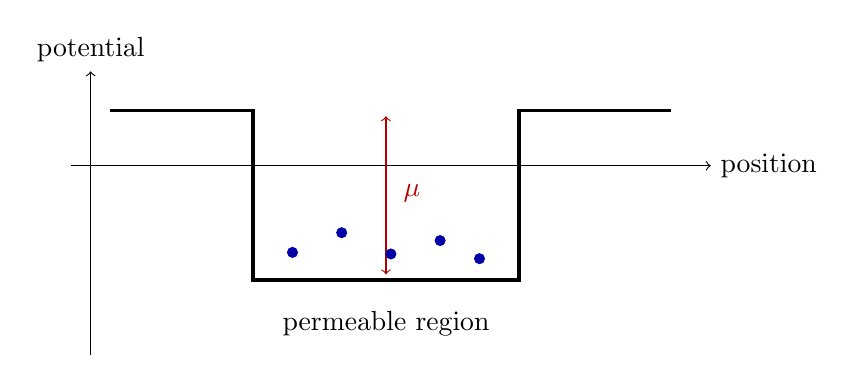
\begin{tikzpicture}[x=1.25cm,y=1.0cm]
\draw[->] (-3.2,0) -- (3.3,0) node[right] {position};
\draw[->] (-3.0,-2.4) -- (-3.0,1.2) node[above] {potential};
\draw[very thick] (-2.8,0.7) -- (-1.35,0.7)
 -- (-1.35,-1.45) -- (1.35,-1.45) -- (1.35,0.7) -- (2.9,0.7);
\draw[<->,red!70!black] (0,0.63) -- (0,-1.38);
\node[right,red!70!black] at (0.08,-0.35) {$\mu$};
\foreach \x/\y in {-0.95/-1.1,-0.45/-0.85,0.05/-1.12,0.55/-0.95,0.95/-1.18}
  \fill[blue!65!black] (\x,\y) circle (2pt);
\node at (0,-2.0) {permeable region};
\end{tikzpicture}
}
\caption{퍼텐셜 오프셋을 바꾸면 입자 수에 대한 선호도가 달라진다. 대정준 앙상블에서는 이 오프셋을 화학 퍼텐셜로 나타낸다.}
\end{figure}

이 사고실험을 통해 화학 퍼텐셜을 구체적으로 이해할 수 있다. 이는 저장고를 기준으로 입자가 하나 더 들어올 때 얻는 에너지 이득이다. 벽을 통과할 수 있는 입자종이 여러 개라면 각 입자종은 고유한 화학 퍼텐셜을 가진다. 밀폐된 상자는 다르다. 그 경우 \(N\)이 고정되고, 화학 퍼텐셜은 저장고와의 교환으로 부과되는 것이 아니라 열역학적으로 추론된다.

\begin{classroomqa}
\audiencequestion{우물의 깊이가 문자 그대로 화학 퍼텐셜인가요?}
\lecturerresponse{이는 화학 퍼텐셜 차이를 직접적으로 구현하는 역학적 방법이다. 내부의 모든 단입자 에너지 준위를 \(\mu\)만큼 낮추면 에너지에 \(-\mu N\)가 더해지고, 따라서 볼츠만 지수에는 \(+\beta\mu N\)가 더해진다. 중요한 것은 화학 퍼텐셜의 차이뿐이다. \lecturetimestamp{00:44:49--00:45:40}}
\end{classroomqa}

입자가 드나들 수 있으므로 분배합에는 모든 입자 수가 포함되어야 한다.
\begin{equation}
\Xi(T,\mu)
=\sum_{N=0}^{\infty}\;\sum_{\mathcal C_N}
\exp\!\left[-\beta E(\mathcal C_N)+\beta\mu N\right].
\label{eq:grand-partition}
\end{equation}
안쪽 합은 \(N\)가 정해진 배치들에 대해 취하고, 바깥쪽 합은 \(N\) 자체에 대해 취한다. 대정준 가중치는 다음처럼 쓸 수도 있다. \(e^{-\beta(E-\mu N)}\)

\begin{figure}[ht]
\centering
\includegraphics[width=0.88\textwidth]{lecture_10_figure_08.png}
\caption{투과성 상자와 입자 수 및 배열에 대한 대정준 합.}
\lectureframe{00:47:15}
\end{figure}

\begin{classroomqa}
\audiencequestion{상자를 밀폐하면 무엇이 달라지나요?}
\lecturerresponse{입자 수의 요동이 멈춘다. 그러면 \(N\)가 고정된 정준 분배함수를 사용한다. 투과성 상자에서는 \(N\)가 열역학적 변수이며, 평균적으로 \(\mu\)에 의해 조절된다. \lecturetimestamp{00:45:42--00:47:50}}
\end{classroomqa}

온도를 고정한 채 \(\mu\)를 바꾸면 보통 밀도는 매끄럽게 변한다. 그러나 임계 온도 아래에서는 밀도가 급격히 뛰어오를 수 있다. 이것이 우리가 살펴보려는 유체 현상이다. 이를 미시적으로 구현하려면 입자에 두 가지 성질이 필요하다. 같은 자리를 동시에 차지할 수 없어야 하고, 단거리에서 서로 끌어당겨야 한다.

\section{스핀을 격자 기체로 바꾸기}

격자는 그대로 두고 두 상태를 새롭게 해석하자. 점유수를 다음과 같이 정의한다.
\begin{equation}
n_i=\frac{1+\sigma_i}{2}
=
\begin{cases}
0,&\sigma_i=-1,\\
1,&\sigma_i=+1.
\end{cases}
\label{eq:occupation-map}
\end{equation}
빈 사이트의 스핀은 아래쪽이고, 점유된 사이트의 스핀은 위쪽이다. \(n_i\)는 0 또는 1만 가능하므로 이중 점유는 금지된다. 따라서 격자 자체가 하드코어를 제공한다.

\begin{figure}[ht]
\centering
\includegraphics[width=0.84\textwidth]{lecture_10_figure_04.png}
\caption{격자 기체와의 대응은 \(\sigma=-1\)를 빈 격자점으로 두는 데서 시작한다. 그러면 \(\sigma=+1\)는 점유된 격자점이다.}
\lectureframe{00:53:45}
\end{figure}

빈 격자, 즉 모든 사이트가 \(\sigma=-1\)인 상태에서 시작하자. 모든 결합이 정렬되어 있고 에너지는 \(-J\)이다. 이 상수 진공 에너지는 빼도 된다. 이제 2차원에서 한 사이트에 입자 하나를 놓자. 해당 스핀은 \(+1\)로 뒤집히며 결합 네 개가 끊어진다. 결합 하나를 끊는 데 \(2J\)가 들므로,
\begin{equation}
\Delta E_1=4(2J)=8J.
\label{eq:one-particle-cost}
\end{equation}
서로 멀리 떨어진 입자 두 개는 결합 여덟 개를 끊고 \(16J\)의 에너지가 든다. 두 입자가 이웃한 사이트를 차지하면 두 입자 사이의 결합은 다시 정렬된다. 경계 결합 여섯 개만 끊어지므로 에너지 비용은
\begin{equation}
\Delta E_{2,\rm adjacent}=6(2J)=12J.
\end{equation}
이다. 따라서 두 입자를 가까이 가져오면 에너지가 다음만큼 낮아진다.
\begin{equation}
16J-12J=4J.
\label{eq:lattice-attraction}
\end{equation}
판서 중에는 이 절감량을 처음에 \(2J\)라고 설명했다가 바로잡았다. 공유 결합 하나가 경계에서 끊긴 결합의 기여 두 개를 없애므로 인력은 \(4J\)이다.

\begin{figure}[ht]
\centering
\includegraphics[width=0.84\textwidth]{lecture_10_figure_05.png}
\caption{2차원에서의 결합 수: 고립된 입자 하나에는 \(8J\)의 에너지가 들고, 멀리 떨어진 입자 두 개에는 \(16J\)의 에너지가 들며, 서로 인접한 입자 두 개에는 \(12J\)의 에너지가 든다.}
\lectureframe{01:00:25}
\end{figure}

이제 격자 기체는 필요한 두 가지 분자적 성질을 모두 갖췄다. 이진 점유가 하드코어 배제를 제공하고, 교환 상호작용이 세기 \(4J\)인 최근접 이웃 인력을 제공한다. 스핀 반전으로 점유 사이트 수가 변하므로 입자 수는 요동할 수 있다.

\subsection{정확한 대수적 대응}

결합 수를 세는 그림만으로도 물리를 파악할 수 있지만, 변수를 정확히 바꾸면 두 모형의 등가성이 더욱 분명해진다. 다음을 대입하자.
\begin{equation}
\sigma_i=2n_i-1
\end{equation}
식~\eqref{eq:ising-hamiltonian}에 대입하면, 결합 하나에 대해
\begin{equation}
\sigma_i\sigma_j
=4n_in_j-2n_i-2n_j+1.
\end{equation}
정규 \(d\)차원 격자에서는
\begin{equation}
\sum_{\langle ij\rangle}(n_i+n_j)=2d\sum_i n_i.
\end{equation}
따라서
\begin{align}
\mathcal H
&=-4J\sum_{\langle ij\rangle}n_in_j
+(4dJ+2h)\sum_i n_i+\text{constant}.
\label{eq:ising-as-lattice-gas}
\end{align}
이를 통상적인 격자 기체 해밀토니안
\begin{equation}
\mathcal H_{\rm lg}
=-\epsilon\sum_{\langle ij\rangle}n_in_j
-\mu\sum_i n_i+\text{constant}.
\label{eq:lattice-gas-hamiltonian}
\end{equation}
과 비교하면 대응 관계는 다음과 같다.
\begin{equation}
\boxed{\epsilon=4J,\qquad
\mu=-(4dJ+2h).}
\label{eq:chemical-potential-map}
\end{equation}

\begin{figure}[ht]
\centering
\includegraphics[width=0.88\textwidth]{lecture_10_figure_09.png}
\caption{입자 에너지 계산 옆에 나타낸 교환항과 자기장 항. 자기장은 가장 가까운 이웃 사이의 인력은 바꾸지 않으면서 삽입 에너지를 바꾼다.}
\lectureframe{01:04:30}
\end{figure}

2차원에서 입자 하나를 고립된 상태로 삽입하면 에너지는 다음만큼 변한다.
\begin{equation}
8J+2h=-\mu.
\end{equation}
\(8J\)는 결합이 끊어진 데서 오고, \(2h\)는 스핀 하나를 \(-1\)에서 \(+1\)로 바꾼 데서 온다. 따라서 \(h\)를 조절하면 인력 \(4J\)를 고정한 채 화학 퍼텐셜을 조절할 수 있다. 교환 에너지의 기준값이 오프셋 \(4dJ\)을 보태므로 자기장은 \(\mu\)와 문자 그대로 같지 않다.

\begin{classroomqa}
\audiencequestion{자기장이 입자 수를 조절한다면, \(h\)는 왜 단순히 화학 퍼텐셜이 아닌가요?}
\lecturerresponse{빈 기준 상태에 비해 입자를 만들면 교환 결합도 끊어진다. 따라서 \(-N\)의 통상적인 계수는 단순히 \(-2h\)가 아니라 \(\mu=-(4dJ+2h)\)이다. 이 오프셋은 \(J\)와 배위수에 따라 달라진다. \lecturetimestamp{01:06:28--01:06:41}}
\end{classroomqa}

밀도는 마찬가지로 간단하다.
\begin{equation}
\rho=\expect{n_i}
=\frac{1+\expect{\sigma_i}}{2}
=\frac{1+m}{2}.
\label{eq:density-map}
\end{equation}
따라서 \(m=-1\)는 빈 격자, \(m=+1\)는 완전히 채워진 격자, \(m=0\)는 반점유 상태다. 전체 입자 수는 \(N_{\rm p}=\sum_i n_i\)이고, 밀도는 \(N_{\rm p}/N\)이다.

\begin{figure}[ht]
\centering
\includegraphics[width=0.90\textwidth]{lecture_10_figure_10.png}
\caption{자기 공존선 옆에 나타낸 밀도 관계식 \(\rho=(1+m)/2\).}
\lectureframe{01:08:25}
\end{figure}

\begin{classroomqa}
\audiencequestion{\((1+m)/2\)는 입자 수인가요, 밀도인가요?}
\lecturerresponse{이는 사이트당 평균 점유수이므로 무차원 격자 밀도다. 전체 사이트 수를 곱하면 기대 입자 수가 된다. 집중량인 밀도와 크기 의존적인 총량을 구별하는 것이 중요하다. \lecturetimestamp{01:06:43--01:09:31}}
\end{classroomqa}

\section{자기 상도가 유체 상도로 바뀌다}

식~\eqref{eq:chemical-potential-map}과 \eqref{eq:density-map}를 사용해 그림~\ref{fig:ising-phase-plane}을 옮겨 해석하자. \(T_c\)보다 높은 온도에서는 \(\mu\)를 바꿔도 밀도가 매끄럽게 변한다. \(T_c\) 아래에서는 공존값을 가로지르면
\begin{equation}
\mu_{\rm coex}=-4dJ
\qquad(h=0)
\label{eq:coexistence-mu}
\end{equation}
밀도가 희박한 기체와 조밀한 액체 사이에서 급격히 바뀐다. \(T_c\)에서는 두 밀도가 합쳐지고 불연속성이 사라진다.

\begin{figure}[ht]
\centering
\includegraphics[width=0.92\textwidth]{lecture_10_figure_11.png}
\caption{이징 공존선을 액체--기체 상도표로 해석한 그림. 기체는 저밀도 쪽에, 액체는 고밀도 쪽에 있으며, 임계 끝점을 돌아 두 상을 연속적으로 연결할 수 있다.}
\lectureframe{01:14:30}
\end{figure}

\begin{figure}[ht]
\centering
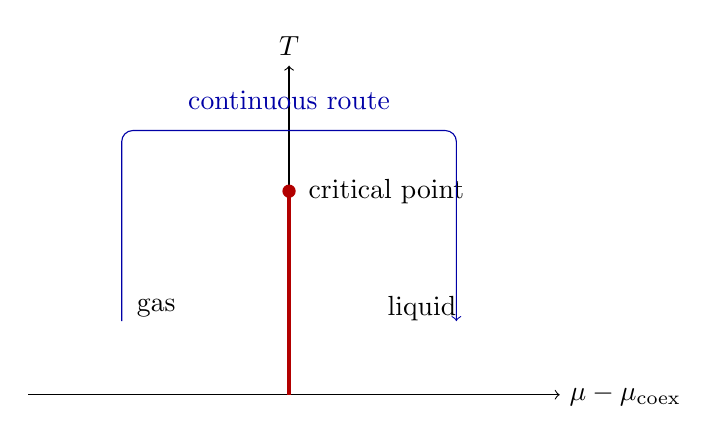
\begin{tikzpicture}[x=1.25cm,y=1.1cm]
\draw[->] (-2.65,0) -- (2.75,0) node[right] {$\mu-\mu_{\rm coex}$};
\draw[->] (0,0) -- (0,3.8) node[above] {$T$};
\draw[very thick,red!70!black] (0,0) -- (0,2.35);
\fill[red!70!black] (0,2.35) circle (2.4pt);
\node[right] at (0.1,2.35) {critical point};
\node at (-1.35,1.0) {gas};
\node at (1.35,1.0) {liquid};
\draw[->,blue!65!black,rounded corners]
 (-1.7,0.85) -- (-1.7,3.05) -- (1.7,3.05) -- (1.7,0.85);
\node[blue!65!black] at (0,3.4) {continuous route};
\end{tikzpicture}
\caption{액체와 기체는 끝점 아래에서는 서로 다른 상이지만, 초임계 영역에서는 두 상을 가르는 특이 경계가 없다.}
\label{fig:liquid-gas-plane}
\end{figure}

이제 익숙한 끓음선을 확인할 수 있다. 압력을 고정한 채 액체를 가열해 공존선을 넘으면 끓음이 일어난다. 온도를 고정한 채 압력이나 화학 퍼텐셜을 바꿔도 같은 경계를 넘을 수 있다. 과열 증기나 과냉각 액체는 평형 공존선 너머로 이어지는 준안정 상태다. 이 상태의 수명을 설명하려면 핵생성 동역학이 필요하며, 이는 여기서 다루는 평형 이론의 범위를 벗어난다.

\begin{classroomqa}
\audiencequestion{과열 증기는 이 상도에 표시되어 있나요?}
\lecturerresponse{평형 상도는 공존 경계를 나타낸다. 과열 상태나 과포화 상태는 준안정 상태다. 임계 액적을 만드는 데 계면 자유 에너지 비용이 들기 때문에, 평형상으로는 맞지 않는 쪽에서도 일시적으로 유지된다. 여기서는 이러한 동역학적 세부 사항을 계산하지 않는다. \lecturetimestamp{01:12:19--01:12:29}}
\end{classroomqa}

\begin{classroomqa}
\audiencequestion{보통 유체에서는 화학 퍼텐셜을 어떻게 바꾸나요?}
\lecturerresponse{퍼텐셜 우물 상자가 이론적으로 제어하기에 가장 간명한 방법이다. 실험실에서는 압력이나 부피를 바꾸거나 저장고와 접촉시키는 경우가 더 많다. 그러면 열역학을 통해 그러한 조절 변수가 화학 퍼텐셜의 변화로 환산된다. \lecturetimestamp{01:12:30--01:13:59}}
\end{classroomqa}

\begin{classroomqa}
\audiencequestion{밀도가 변할 때 분자 퍼텐셜 \(J\)도 바뀌나요?}
\lecturerresponse{아니다. 물질이 고정되어 있다면 \(J\)는 단거리 인력을 나타내며 이 모형에서는 일정하게 유지된다. \(\mu\)를 바꾸면 점유된 사이트 수가 변하고, 따라서 분자 간 거리의 분포가 달라진다. \(J\)를 바꾸는 것은 미시적 물질이나 상호작용 자체를 바꾸는 일이다. \lecturetimestamp{01:14:50--01:15:41}}
\end{classroomqa}

\begin{classroomqa}
\audiencequestion{임계 온도는 보통 말하는 끓는점과 같은 것인가요?}
\lecturerresponse{아니다. 끓는점은 선택한 압력에서 정해지므로 압력이 바뀌면 공존 곡선을 따라 이동한다. 임계 온도는 그보다 높은 온도에서 액체와 기체를 가르는 상경계가 더 이상 존재하지 않게 되는 유일한 종점이다. 이 격자 기체 설명에서는 압력을 명시적으로 유도하지 않았다. \lecturetimestamp{01:15:42--01:17:02}}
\end{classroomqa}

이제 핵심 결과를 말할 수 있다. 이징 자석과 격자 기체는 단지 비슷한 상도를 그리는 데 그치지 않는다. 변수와 매개변수를 바꾸면 두 계의 분배함수는 서로 일치한다. 한쪽의 모든 특이한 열역학적 성질은 다른 쪽에도 대응하는 성질이 있다.
\begin{equation}
\begin{array}{c|c}
\text{Ising magnet} & \text{lattice gas}\\ \hline
\sigma_i=\pm1 & n_i=0,1\\
m=\expect{\sigma} & \rho=(1+m)/2\\
h & \mu=-(4dJ+2h)\\
\text{aligned exchange} & \text{nearest-neighbor attraction}\\
h=0,\ T<T_c & \text{liquid--gas coexistence}\\
(T_c,0) & \text{critical endpoint}
\end{array}
\label{eq:ising-fluid-dictionary}
\end{equation}

\section{임계 지수와 보편성}

임계점 가까이에서는 열역학량에 멱법칙 특이성이 나타나는 경우가 많다. 환산 온도를
\begin{equation}
t=\frac{T-T_c}{T_c},
\end{equation}
정의하면, 개략적으로 다음과 같이 쓴다.
\begin{equation}
m\sim(-t)^{\beta_{\rm crit}},
\qquad
\chi\sim |t|^{-\gamma},
\qquad
\xi\sim |t|^{-\nu}.
\label{eq:critical-exponents}
\end{equation}
여기서 \(\beta_{\rm crit}\)는 임계 지수이지 역온도가 아니다. 평균장 이론은 \(\beta_{\rm crit}=1/2\)를 주지만, 상한 임계 차원 아래에서는 요동 때문에 지수가 달라진다.

임계 지수가 정수일 필요는 없다. 모두 무리수인 것도 아니다. 2차원 이징 모형에는 잘 알려진 정확한 유리수 임계 지수가 여럿 있지만, 3차원 이징 모형의 값은 이론과 계산을 통해 높은 정밀도로 정해지는 비자명한 수다. 여기서 얻을 수 있는 확실한 교훈은 임계 지수가 일반적으로 기초적인 차원 분석만으로 정해지지 않는다는 것이다.

더욱 놀랍게도 임계 지수는 미시적 세부 사항에 의해 정해지지 않는 경우가 많다. 공간 차원, 질서변수 대칭성, 그리고 충분히 짧은 상호작용 범위가 같은 계들은 동일한 장거리 임계 이론으로 흐를 수 있다. 이들은 하나의 \emph{보편성} 부류에 속한다. 단축성 자석과 보통 액체--기체 계의 임계점은 둘 다 스칼라 질서변수 하나를 가지며, 같은 차원에서는 이징 보편성 부류에 속한다.

\begin{classroomqa}
\audiencequestion{}보편성 부류는 유한하거나 이산적인 목록인가요?\lecturerresponse{
보편성 부류는 여러 가지가 있으며, 차원과 대칭성, 보존 법칙, 상호작용 범위 및 그 밖의 장거리 특성에 따라 분류된다. 익숙한 경우에는 고정점과 임계 지수 집합이 이산적이지만, 임계 지수가 연속적으로 변하는 계도 있다. 목록이 유한하다고 단정하기는 어렵다. 여러 미시적으로 다른 계가 같은 장거리 특성을 공유한다는 것이 안전하게 말할 수 있는 내용이다. \lecturetimestamp{01:18:50--01:19:38}}
\end{classroomqa}

\begin{classroomqa}
\audiencequestion{액체와 기체가 공존한다면 실제 용기 안에서 둘을 가르는 것은 무엇인가요?}
\lecturerresponse{계면이 둘을 가른다. 표면 장력은 계면 면적을 늘리는 데 에너지 비용을 부과하고, 중력은 수직 방향의 화학 퍼텐셜 기울기를 만들어 보통 밀도가 높은 액체를 기체 아래에 놓는다. 중력을 무시할 수 있으면 계면의 모양은 표면 장력과 경계 조건에 더 직접적으로 좌우된다. \lecturetimestamp{01:19:40--01:21:18}}
\end{classroomqa}

\begin{classroomqa}
\audiencequestion{이 그림에서는 기화열이 어디에 나타나나요?}
\lecturerresponse{임계점 아래에서 1차 공존선을 가로지르면 일반적으로 잠열이 수반됩니다. 임계 종점에 가까워질수록 두 상이 서로 같아지므로 기화열은 0에 가까워집니다. 이 강의에서는 상 구조를 설명하지만 잠열을 계산하지는 않습니다. \lecturetimestamp{01:21:19--01:22:18}}
\end{classroomqa}

\begin{classroomqa}
\audiencequestion{초전도 소자 같은 장치에서 상전이를 민감한 검출기로 활용할 수 있나요?}
\lecturerresponse{네. 상전이 부근에서는 작은 섭동이 큰 반응을 일으키거나 상태 변화를 촉발할 수 있습니다. 실제 검출기는 이러한 민감도를 활용하지만, 관련 질서 매개변수와 동역학은 이징 모형의 경우와 다를 수 있습니다. \lecturetimestamp{01:22:19--01:24:05}}
\end{classroomqa}

이로써 통계역학 강의가 끝납니다. 엔트로피와 평형에서 시작해 분배함수와 기체를 거쳐, 자석과 유체가 동일한 임계 현상을 서로 다르게 기술할 수 있음을 보이는 데 이르렀습니다.

\section{강의 후 토론: 미세 조정과 선택}

정식 강의가 끝난 뒤에도 대화는 약 40분간 이어졌습니다. 이 내용을 보존할 가치는 있지만, 앞서 제시한 유도와 혼동해서는 안 됩니다. 이제 주제는 격자 기체가 아닙니다. 우주론에서 미세 조정의 논리와 인류 원리적 선택을 신중하게 사용하는 문제입니다.

\subsection{작은 수라고 해서 저절로 미세 조정된 것은 아니다}

\emph{인류 원리}라는 표현의 모든 쓰임을 단번에 정리해 주는 문장은 없습니다. 유용한 출발점은 실질적인 관점입니다. 이론이 실현된 환경을 여러 가지 허용한다면, 관측은 관측자가 생겨날 수 있는 환경이 일부에 한정된다는 사실을 조건으로 삼습니다. 이런 조건부 진술은 합리적일 수 있습니다. 하지만 앙상블이나 선택 조건, 또는 대안들을 물리적으로 의미 있게 만드는 메커니즘 없이 이를 내세우면 공허해집니다.

선택을 논하기 전에 작은 매개변수와 미세 조정된 매개변수를 구별해야 합니다. 안정적인 동역학적 메커니즘이 어떤 값을 특별한 값으로 이끌기 때문에 수가 작을 수 있습니다. 미세 조정이란 관측된 값이 서로 독립적인 기여들 사이의 극도로 정밀한 균형을 필요로 하는 것처럼 보이는데, 그 균형을 지켜 주는 복원 메커니즘이나 대칭성이 알려져 있지 않은 경우를 뜻합니다.

\begin{classroomqa}
\audiencequestion{인류 원리를 명확하게 진술할 수 있나요?}
\lecturerresponse{정당화할 수 있는 사용법은 신비주의가 아니라 조건부 진술입니다. 서로 다른 매개변수를 가진 물리적으로 실현된 환경이 많다면, 우리와 같은 존재가 관측하는 환경은 관측자가 존재할 수 있는 부분집합에서 뽑힙니다. 그렇다고 해서 이 진술만으로 환경이 생성되거나 그 확률이 정해지는 것은 아닙니다. 그런 일은 기저 물리학이 설명해야 합니다. \lecturetimestamp{01:25:45--01:26:13}}
\end{classroomqa}

우주상수가 이 논의를 이끄는 사례입니다. 관측된 우주상수의 크기는 진공 에너지에 대한 순진한 양자장론적 기여와 비교하면 놀라울 만큼 작습니다. 문제는 최종값이 작다는 데만 있지 않습니다. 받아들여지는 저에너지 피드백 메커니즘이 결과를 관측값 쪽으로 조정하지 못하는 상황에서, 큰 항 여러 개가 엄청난 정밀도로 상쇄되어야 하는 것처럼 보인다는 점이 문제입니다.

\subsection{비행선과 잠수함}

부력에 관한 두 사례를 보면 이 차이가 분명해집니다. 비행선은 평균 밀도가 주변 공기의 밀도와 같아지는 고도에서 뜹니다. 공기의 밀도는 고도가 높아질수록 감소합니다. 비행선이 상승하면 바깥 공기의 밀도가 낮아져 비행선은 내려가려 하고, 하강하면 바깥 공기의 밀도가 높아져 비행선은 상승하려 합니다. 밀도를 일치시키는 값은 수치상으로 미세하게 조정되어 있을 수 있지만, 대기의 밀도 구배가 복원 피드백을 제공합니다. 이 평형은 동역학적으로 설명됩니다.

밀도가 깊이에 따라 거의 변하지 않는 물속에서 중성 부력을 갖는 잠수함은 다릅니다. 잠수함의 평균 밀도가 주변 물의 밀도와 우연히 같더라도, 그 일치를 설명해 줄 만한 깊이 의존적 복원 메커니즘은 없습니다. 아주 작은 불일치만 있어도 잠수함은 상승하거나 가라앉습니다. 중성 부력을 얻으려면 밸러스트와 적재물을 정밀하게 조절해야 합니다. 이 잔차를 설명하는 제어 시스템이나 설계 메커니즘이 없다면, 그 작은 잔차는 미세 조정된 것입니다.

\begin{figure}[ht]
\centering
\resizebox{\linewidth}{!}{%
\begin{tikzpicture}[>=Latex]
\begin{scope}[xshift=-3.8cm]
\shade[top color=blue!5,bottom color=blue!28] (-2.5,-2.2) rectangle (2.5,2.2);
\draw[very thick,rounded corners=18pt,fill=yellow!35]
  (-1.15,0) ellipse (1.15 and 0.55);
\draw[thick] (0,-0.55) -- (0,-1.05);
\draw[thick,fill=gray!20] (-0.45,-1.05) rectangle (0.45,-1.38);
\draw[->,red!70!black,thick] (1.65,1.45) -- (1.65,0.55)
 node[midway,right] {restoring};
\draw[->,red!70!black,thick] (-1.65,-1.45) -- (-1.65,-0.55)
 node[midway,left] {restoring};
\node at (0,2.55) {\textbf{Blimp: density gradient}};
\node[align=center] at (0,-2.75) {displacement changes\\the buoyant imbalance};
\end{scope}
\begin{scope}[xshift=3.8cm]
\shade[top color=cyan!10,bottom color=blue!45] (-2.5,-2.2) rectangle (2.5,2.2);
\draw[very thick,fill=gray!35,rounded corners=12pt]
  (-1.45,-0.25) -- (1.1,-0.25) arc (-90:90:0.38)
  -- (-1.45,0.51) -- cycle;
\draw[thick] (-0.25,0.51) -- (-0.25,0.85) -- (0.35,0.85) -- (0.35,0.51);
\draw[->,red!70!black,thick] (1.65,0.15) -- (1.65,1.35)
 node[midway,right] {rise};
\draw[->,red!70!black,thick] (-1.65,0.15) -- (-1.65,-1.35)
 node[midway,left] {sink};
\node at (0,2.55) {\textbf{Submarine: nearly uniform density}};
\node[align=center] at (0,-2.75) {no depth-dependent feedback\\protects neutral buoyancy};
\end{scope}
\end{tikzpicture}
}
\caption{작은 잔차는 동역학적으로 안정적일 수도 있고 실제로 미세 조정된 것일 수도 있습니다. 비행선에는 복원 피드백이 있지만, 이상화한 잠수함은 평균 밀도를 물의 밀도에 맞춰야 합니다.}
\label{fig:blimp-submarine}
\end{figure}

\begin{classroomqa}
\audiencequestion{중성 부력이 관측되었다면 잠수함 승무원은 왜 설명을 요구해야 하나요?}
\lecturerresponse{밸러스트를 조절하는 메커니즘이 없다면, 서로 독립적인 두 밀도의 일치를 보호하는 대칭성도 환경 피드백도 없기 때문입니다. 문제는 그 일치가 논리적으로 가능한가가 아니라, 계가 왜 매개변수 공간의 그토록 좁은 영역에 놓여 있는가입니다. \lecturetimestamp{01:35:05--01:36:25}}
\end{classroomqa}

\subsection{여러 영역과 조건부 관측}

이제 평균 밀도가 서로 다른 잠수함을 엄청나게 많이 만들어 내는 과정이 있다고 상상해 봅시다. 대부분은 가라앉거나 떠오르고, 극히 일부만 수면과 바닥 사이의 거주 가능 영역에 오랫동안 남습니다. 살아남은 잠수함 가운데 하나에서 필연적으로 살아가는 관측자는 중성 부력에 가까운 값을 측정하더라도 놀랄 이유가 없습니다. 관측자가 존재하기 위해 필요한 조건에 따라 관측 결과가 선택되기 때문입니다.

이 논리에는 두 가지 요소가 필요합니다.
\begin{enumerate}
\item 상상 속에서만 존재하는 대안이 아니라 여러 대안을 실제로 실현하는 물리적 과정;
\item 관측이 제한된 부분집합에서만 이루어지는 이유를 설명하는 선택 조건.
\end{enumerate}
선택은 생성 메커니즘을 대체하지 않습니다. 앙상블이 존재할 때 관측자가 무엇을 측정할지에 대한 조건부 확률을 바꿉니다.

\begin{classroomqa}
\audiencequestion{충분히 큰 표본의 어딘가에서는 드문 일이 일어난다는 주장에 불과한가요?}
\lecturerresponse{그것은 논리의 절반에 불과합니다. 나머지 절반은 관측 조건화입니다. 관측자는 모든 영역에서 균일하게 표집되는 것이 아니라, 자신이 존재할 수 있는 영역에서만 표집됩니다. 완전한 제안이라면 영역에 대한 측도와 영역이 어떻게 생성되는지에 관한 물리적 설명도 필요합니다. \lecturetimestamp{01:39:19--01:40:36}}
\end{classroomqa}

진공 에너지에 적용하면, 큰 음의 우주상수는 우주를 지나치게 빠르게 재수축하게 할 수 있고, 충분히 큰 양의 값은 물질이 은하로 응집하는 것을 막을 수 있습니다. 관측된 값은 구조가 오래 유지될 수 있는 좁은 범위 안에 있습니다. 이는 가능한 선택 조건을 제시하지만, 우주상수 분포를 유도하지는 않습니다.

양자장론은 미세 조정 문제를 더합니다. 서로 다른 장과 에너지 규모에서 오는 진공 기여는 각각 관측된 잔차보다 훨씬 큽니다. 이 항들이 거의 완벽하게 상쇄된다면, 그 결과는 스스로 균형을 바로잡는 비행선보다 세심하게 균형을 맞춘 잠수함에 가깝습니다. 이 비유는 논리적 문제를 드러내기 위한 것이지, 그 해답을 제시하기 위한 것은 아닙니다.

\begin{classroomqa}
\audiencequestion{한 매개변수의 변화가 다른 여러 매개변수의 변화로 상쇄될 수 있나요?}
\lecturerresponse{네. 가능한 집합은 한 축의 좁은 구간이 아니라 여러 차원으로 이루어진 매개변수 공간의 얇은 곡면일 수 있습니다. 서로 상관된 변화가 구조를 유지할 수 있지만, 그러면 실현된 매개변수들이 왜 그 곡면 가까이에 놓이는지, 또 기저 이론이 그 곡면에 어떤 측도를 부여하는지가 문제가 됩니다. \lecturetimestamp{01:45:10--01:46:19}}
\end{classroomqa}

\begin{figure}[ht]
\centering
\begin{tikzpicture}[x=1.3cm,y=1.05cm,>=Latex]
\draw[->] (-3.2,0) -- (3.4,0) node[right] {$\lambda_1$};
\draw[->] (0,-2.5) -- (0,2.65) node[above] {$\lambda_2$};
\fill[gray!12] (-3,-2.25) rectangle (3.1,2.3);
\draw[very thick,blue!65!black]
 (-2.8,-1.55) .. controls (-1.3,-0.75) and (0.15,0.05) .. (2.85,1.55);
\draw[very thick,blue!25]
 (-2.8,-1.25) .. controls (-1.3,-0.45) and (0.15,0.35) .. (2.85,1.85);
\fill[blue!15,opacity=.65]
 (-2.8,-1.55) .. controls (-1.3,-0.75) and (0.15,0.05) .. (2.85,1.55)
 -- (2.85,1.85) .. controls (0.15,0.35) and (-1.3,-0.45) .. (-2.8,-1.25) -- cycle;
\node[blue!65!black,rotate=28] at (1.3,0.95) {viable band};
\foreach \x/\y in {-2.4/1.45,-1.7/-1.8,-0.9/1.8,0.3/-1.45,1.2/1.85,2.4/-0.8}
  \fill[red!65!black] (\x,\y) circle (2pt);
\fill[green!45!black] (0.55,0.58) circle (2.8pt);
\node[green!35!black,right] at (0.65,0.55) {observed domain};
\end{tikzpicture}
\caption{매개변수가 여러 개일 때 거주 가능성이나 구조적 실현 가능성은 한 매개변수의 좁은 구간이 아니라, 서로 상관된 얇은 띠에 놓일 수 있습니다. 선택은 관측을 그 띠 안으로 제한하지만 매개변수 분포를 만들어 내지는 않습니다.}
\label{fig:viable-parameter-band}
\end{figure}

\subsection{풍경 제안과 그 불확실성}

대안을 만들어 내는 원천으로 제안된 것 가운데 하나는 많은 준안정 진공을 가진 이론이며, 서로 다른 우주론적 영역에 각기 다른 진공이 채워질 수 있습니다. 끈 이론의 풍경 구상과 영원한 급팽창 시나리오가 그 예지만, 구체적인 실현 방식과 확률 측도는 여전히 불확실합니다. 강의에서는 이를 확립된 사실이 아니라 가능성으로 제시합니다.

우주상수가 정확히 영이 되도록 대칭성이 강제한다면, 이는 더 통상적인 설명이 될 것이다. 문제는 관측된 가속 팽창에 작지만 영이 아닌 값이 대응한다는 점이다. 자연스럽게 정확히 영을 만드는 메커니즘이 있다고 해서 아주 작은 잔여값까지 자동으로 설명되는 것은 아니다. 대칭성을 깨면 미세 조정 문제가 다시 생길 수 있다. 여기서 잠수함의 비유가 다시 떠오른다. 밧줄로 잠수함을 원하는 깊이에 고정할 수는 있지만, 그렇다면 밧줄은 당연한 것으로 가정할 것이 아니라 밝혀내야 할 메커니즘이다.

\begin{classroomqa}
\audiencequestion{매개변수를 매우 정밀하게 측정하면 불확정성 원리에 위배되나요?}
\lecturerresponse{아닙니다. 불확정성 관계는 특정한 비가환 관측량의 쌍에 적용됩니다. 결합 상수나 진공 매개변수는 통제되지 않는 관측량의 정준 켤레가 아니어도 정확히 정해진 값을 가질 수 있습니다. 정밀하다는 사실 자체는 불확정성 원리의 역설이 아닙니다. \lecturetimestamp{01:49:21--01:49:36}}
\end{classroomqa}

\begin{classroomqa}
\audiencequestion{인류 원리는 값이 왜 그런지 설명하나요, 아니면 관측자에게 그 값이 필요하다는 말만 되풀이하나요?}
\lecturerresponse{선택만으로는 동역학적 설명이 되지 않습니다. 정당한 역할은 물리적으로 실현된 앙상블에서 조건부 확률을 바꾸는 것입니다. 앙상블이나 측도, 검증 가능한 귀결 없이 사용하면 설명이 아니라 이름표에 그칠 위험이 있습니다. \lecturetimestamp{01:49:37--01:50:21}}
\end{classroomqa}

\subsection{입자물리학의 적당한 정도의 우연의 일치}

생명과 관련된 모든 매개변수가 똑같이 이례적인 정도로 미세 조정되어 있는 것은 아니다. 우리가 익히 아는 물질은 광자, 전자, 가벼운 쿼크와 강한 상호작용에 의존한다. 중성미자는 우주론에 영향을 미치지만 원자를 직접 결합시키는 역할을 하지는 않는다. 양성자--중성자 질량 차이는 특히 중요하다. 중성자가 양성자보다 약간 더 무겁기 때문에 고립된 중성자는 붕괴할 수 있고, 보통의 수소는 안정하다. 질량의 대소 관계가 충분히 반대로 바뀐다면 핵화학은 근본적으로 달라질 것이다.

전자 질량과 미세 구조 상수도 원자 크기와 결합 에너지를 정합니다. 이 값들이 크게 변하면 화학도 달라집니다. 이는 의미 있는 민감도에 관한 진술이지만, 작은 변화가 있을 때마다 상상 가능한 모든 복잡한 형태가 불가능해진다는 주장으로 부풀려서는 안 됩니다. 우주상수 문제에 비하면 이런 우연의 일치 가운데 상당수는 완만하며 다른 매개변수들과 상관되어 있습니다.

약전기력 척도와 관련된 계층 문제도 대표적인 자연성 문제입니다. 추가 구조가 보호해 주지 않는 한, 복사 보정 때문에 기본 스칼라 질량은 높은 에너지 척도에 민감해지는 경향이 있습니다. 이 문제의 위상과 해석은 진공 에너지 문제와 다르며, 둘 중 어느 것도 구호로 축약해서는 안 됩니다.

\begin{classroomqa}
\audiencequestion{양성자---중성자 질량 차이를 바꾸면 실제로 보통 물질에 영향이 있나요?}
\lecturerresponse{네. 관측된 질량 순서는 안정한 수소를 가능하게 하고 핵 전반의 베타 안정성을 좌우합니다. 작은 변화도 핵종의 양과 항성의 연소 과정을 재편할 수 있습니다. 정밀한 분석을 하려면 다른 모든 값을 고정한 채 하나의 수만 바꾸는 대신, 서로 결합된 매개변수들을 일관되게 변화시켜야 합니다. \lecturetimestamp{01:51:47--01:53:08}}
\end{classroomqa}

\begin{classroomqa}
\audiencequestion{전자 질량과 미세 구조 상수는 어떤 역할을 하나요?}
\lecturerresponse{이들은 대표적인 원자 에너지 척도와 길이 척도를 정합니다. 개략적으로 \(E_{\rm atom}\sim \alpha^2m_e\), \(a_0\sim(\alpha m_e)^{-1}\)이며 단위는 \(\hbar=c=1\)입니다. 크게 변하면 화학의 구조도 달라지겠지만, 정확히 어떤 범위가 가능한지는 여러 차원에 걸친 문제입니다. \lecturetimestamp{01:53:09--01:54:12}}
\end{classroomqa}

\subsection{의견 차이, 시간 변화, 검증}

토론은 잠시 급팽창에 대한 비판과 정밀 우주론 데이터의 해석으로 넘어갑니다. 이러한 역사적 의견 차이는 수사로 종결된 것처럼 다루지 말고, 의견 차이로 제시해야 합니다. 급팽창에는 현상론적으로 성공한 예측이 있고 여러 모형이 있지만, 초기 조건과 측도, 검증 가능성에 관한 질문은 여전히 활발히 논의되고 있습니다. 데이터는 모형을 제약하지만, 대화 중에 실험을 한 번 언급한다고 해서 전체 이론 체계가 결론 나는 것은 아닙니다.

\begin{classroomqa}
\audiencequestion{우주상수가 상수가 아니라 시간에 따라 천천히 변할 수 있나요?}
\lecturerresponse{동역학적 암흑 에너지 장은 시간에 따라 변하는 가속 팽창을 일으킬 수 있습니다. 하지만 이 경우에도 퍼텐셜과 초기 조건을 도입해야 하며, 이들 역시 설명되어야 합니다. 관측에 따르면 상태 방정식은 우주상수의 경우에 가까운 값으로 제한됩니다. 강의 당시의 논의에서는 시간에 따른 유의미한 변화가 필요하다는 증거가 없었습니다. \lecturetimestamp{01:57:17--01:59:19}}
\end{classroomqa}

\begin{classroomqa}
\audiencequestion{인류 원리적 선택 자체가 서로 다른 우주나 영역을 핵생성하나요?}
\lecturerresponse{아닙니다. 선택은 실현된 영역 가운데 어떤 곳에 관측자가 존재할 수 있는지를 말할 뿐, 그 영역을 만들어 내지는 않습니다. 영역을 생성하려면 급팽창 과정에서의 진공 전이와 같은 별도의 우주론적 메커니즘이 필요합니다. \lecturetimestamp{01:59:20--01:59:42}}
\end{classroomqa}

인과적 순서는 분명해야 합니다.
\begin{equation}
\begin{gathered}
\text{laws and initial conditions}\\[-0.15em]
\downarrow\\[-0.15em]
\text{physical environments}\\[-0.15em]
\downarrow\\[-0.15em]
\text{observers and observations}
\end{gathered}
\end{equation}
관측자가 과거로 거슬러 올라가 법칙을 결정하는 것은 아닙니다. 실현된 환경들에서 뽑힌 관측자가 무엇을 측정할 가능성이 큰지 물을 때 조건화가 들어갑니다.

따라서 과학적 질문은 이 표현이 철학적이거나 정치적이거나 종교적으로 들리는지가 아닙니다. 제안에 정의된 물리적 앙상블과 계산 가능하거나 적어도 제약할 수 있는 측도, 그리고 대안과 구별할 수 있는 귀결이 있는지가 관건입니다. 다중 진공 우주론에서 논의되는 가능한 신호로는 거품 영역 사이의 충돌 흔적이 있습니다. 그런 신호는 신뢰성 있게 예측하기 어렵고, 강의 당시 논의에서는 우주 마이크로파 배경에서 확립된 신호가 없었습니다. 쉽게 검증할 방법이 없다는 점은 심각한 한계입니다. 그렇다고 그 생각을 참이라고 단정하거나 기저의 미세 조정 문제를 무시해도 된다는 뜻은 아닙니다.

\begin{classroomqa}
\audiencequestion{선택 논증을 과학 이론으로 만들려면 무엇이 필요한가요?}
\lecturerresponse{대안을 생성하는 메커니즘과 확률 측도 또는 이를 통제할 수 있는 대안, 그리고 관측 가능한 귀결이 필요합니다. 거품 충돌 신호는 가능한 연구 경로 가운데 하나지만, 신호가 없거나 모호하다는 사실은 검증 가능성의 문제가 얼마나 까다로운지 보여 줍니다. \lecturetimestamp{02:02:31--02:04:12}}
\end{classroomqa}

강의 후 대화는 이러한 절제된 관점으로 끝납니다. 미세 조정은 설명이 빠져 있을 수 있다는 증거입니다. 대칭성, 동역학적 조정, 환경적 선택은 논리적으로 서로 다른 설명 후보입니다. 선택은 합리적일 수 있지만, 그 가정과 한계를 명확히 밝힌 물리적 설명의 한 요소로서만 그렇습니다.
